
\chapter{Beugung am Gitter}
\label{v:10}

In diesem Versuch benutzen Sie den Effekt der Beugung von Licht an einem optischen Gitter, um die Spektrallinien von Quecksilber zu betrachten, sowie die Wellenl"ange der gr"unen Linie zu messen.\\

%------------------------------------------------
\section{Stichworte}
%------------------------------------------------

Koh"arenz; Interferenz; Huygens'sches Prinzip; Gitterkonstante; Interferenzfilter; Beugung am Gitter.
%
%------------------------------------------------
\section{Literatur}
%------------------------------------------------

Gehrtsen, Kapitel 10.1.1-10.1.3, 10.1.12
%

%------------------------------------------------
\section{Anwendungsbeispiele}
%------------------------------------------------

Beugung begrenzt Aufl�sungsverm�gen optischer Ger�te, Spektroskopie, genaue L�ngenmessung, Definition des Meters.

%------------------------------------------------
\section{Theoretischer Hintergrund}
%------------------------------------------------

Die Kenntnis des Aufbaus der Atome geh�rt heute zu den gesicherten Bestandteilen von Physik und Chemie und erm�glicht ein Verst�ndnis der Bindung in Molek�len und Festk�rpern. F�r die Aufkl�rung des Atombaus war die genaue Vermessung des von Atomen ausgesandten Lichtes von ganz wesentlicher Bedeutung.\\
Angeregte Atome senden Licht in Form von Spektrallinien aus, die f�r den Aufbau der �u�eren Elektronenschalen und die chemischen Eigenschaften charakteristisch sind. Das einfachste Atom ist das Wasserstoffatom mit der bekannten Linienfolge der Balmerserie. Das im Periodensystem folgende Heliumatom besitzt zwei Elektronen, die wegen des
Elektronenspins auf verschiedene Weise koppeln k�nnen. Es ist interessant zu beobachten, dass das Spektrum der Spektrallinien des Quecksilberatoms mit seinen 80 Elektronen dem Spektrum des Heliumatoms in gewisser Weise �hnlich ist und dass man charakteristische Unterschiede auf die Relativit�tstheorie zur�ckf�hren kann.\\
Das im Versuch vorgestellte Beugungsgitter ist ein einfaches, aber doch recht leistungsf�higes Ger�t zur Sichtbarmachung von Spektrallinien und zur Vermessung von Wellenl�ngen.

\subsection{Interferenz}

Der Begriff der Interferenz bezeichnet die "Uberlagerung von zwei Wellenz"ugen. Je nachdem, ob die Auslenkung der beiden Wellen dasselbe Vorzeichen haben oder unterschiedliche, addieren oder subtrahieren sich ihre Auslenkungen zur "uberlagerten Welle. Man spricht dann von \textit{konstruktiver} oder \textit{destruktiver} Interferenz.\\
Damit ein sowohl r"aumlich (z.B. auf einem Schirm) als auch zeitlich stabiles Interferenzmuster entsteht, m"ussen die zwei oder mehr "uberlagerten Wellen \textit{koh"arent} sein. Das ist dann der Fall, wenn die Zeitabh"angigkeit der Amplitude in ihnen bis auf eine Phasenverschiebung die gleich ist. Bei rein harmonischen Wellen (Sinus-f"ormig), wie z.B. Lichtwellen, hei{\ss}t das, dass die Frequenzen "ubereinstimmen m"ussen; die Phasen d"urfen eine konstante Differenz gegeneinander haben.

\subsection{Beugung am Spalt}

Die Beugung von Licht an einem Spalt k"onnen Sie sich leicht mit dem Huygens'schen Bild der Elementarwellen klar machen. Betrachten Sie dabei jeden Punkt des Spaltes als Quelle von elementaren Kugelwellen, die sich in gro{\ss}em Abstand wieder zu einer ebenen Wellenfront "uberlagern. Zur Verinfachung betrachten wir nur die Kugelwellen, die an den Kanten des Spaltes der Breite $d$ entstehen.\\
Betrachten Sie den Spalt unter einem Winkel $\alpha$, so m"ussen die Wellenfronten der beiden Seiten des Spaltes unterschiedlich lange Wege zur"ucklegen, um an Ihr Auge zu gelangen. Dieser \textit{Gangunterschied} betr"agt, wie man Abbildung \ref{fig:Spalt} entnimmt:
\begin{equation}
 \Delta s = d\cdot\sin\alpha\, .
\end{equation}
% Hinweis darauf, dass dies eine N�herung f�r den Fall eines hinreichend gro�en Abstands der Beobachtungsebene zum Gitter ist.

\begin{figure}[ht]
	\centering
		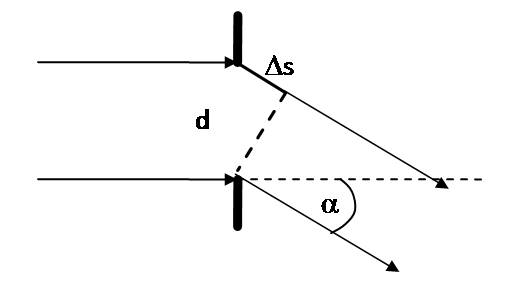
\includegraphics[width=.5\textwidth]{Versuch_9-10/Abbildungen/Spalt.jpg}
	\caption{Beugung am Spalt}
	\label{fig:Spalt}
\end{figure}

\noindent
Betr"agt der Gangunterschied ein ganzzahliges Vielfaches der Wellenl"ange, so tritt konstruktive Interferenz auf, auf dem Schirm sieht man einen hellen Bereich, ein sog. \textit{Interferenzmaximum}. Mit der Definition des Gangunterschiedes ergibt sich also als Bedingung f"ur die Beobachtung eines Interferenzmaximums:
\begin{equation} \label{eq:Interferenzmax}
 \sin\alpha_{max} = \frac{n\cdot\lambda}{d}\, .
\end{equation}
Den Faktor $n$ bezeichnet man die \textit{Ordnung des Maximums}.\\
Offenbar h"angt die Richtung, unter der man ein Interferenzmaximum beobachtet, von der Wellenl"ange des einfallenden Lichtes ab.

\subsection{Beugung am Gitter}

Ein (optisches) Gitter ist ein Anordnung aus vielen schmalen Spalten, die den (konstanten) Abstand $d$ voneinander haben. $d$ bezeichnet man als \textit{Gitterkonstante}.\\
F"ur die Beugung am Gitter gelten dieselben "Uberlegungen wie beim einzelnen Spalt (oder beim Doppelspalt). Aus Gleichung \ref{eq:Interferenzmax} kann man den Abstand $\delta$ zwischen zwei Interferenzmaxima bestimmen. Wenn der Beobachtungsschirm im Abstand $L$ vom Spalt oder Gitter steht, so gilt 
\begin{equation}
 \frac{n\cdot\lambda}{d} = \sin\alpha = \frac{\delta}{L}\, .
\end{equation}
Diesen Zusammenhang kann man benutzen, um aus den messbaren Gr"o{\ss}en $L$ und $\delta$, mit Kenntniss deGitterkonstante $d$, die Wellenl"ange des einfallenden Lichtes zu messen:
\begin{equation}
 \lambda = \delta\cdot\frac{d}{L}\, .
\end{equation}


%------------------------------------------------
\section{Fragen zur Vorbereitung}
%------------------------------------------------

\begin{enumerate}
 %
 \item Was soll heute im Praktikum gemessen werden? Warum?
 %
 \item Was besagt das Huygens'sche Prinzip?
 %
 \item Was ist Interferenz?
 %
 \item Welche Bedingungen m"ussen f"ur die Beobachtung von Interferenzerscheinungen erf"ullt sein?
 %
 \item Was bezeichnen die Gitterkonstante und der Gangunterschied?
 %
 \item Wird am Gitter rotes oder blaues Licht st"arker abgelenkt?
 %
 \item Welche Gr"o{\ss}e wird im Praktikum gemessen, welche Gr"o{\ss}e wird daraus berechnet?
 %
\end{enumerate}

%------------------------------------------------
\section{Durchf�hrung} 
%------------------------------------------------

Das von einer Hg-Lampe erzeugte Licht wird mittels einer Kondensorlinse auf einen engen Spalt fokussiert und mittels einer zweiten Linse L2 parallel gemacht. Ein Gr�nfilter l�sst die gr�ne Spektrallinie des Hg durch. Auf diese Art wird ein koh�rentes, paralleles, nahezu monochromatisches Lichtb�ndel erzeugt, mit dem ein Strichgitter der Gitterkonstanten g beleuchtet wird.

\begin{enumerate}
 %
 \item Bestimmen Sie die Gitterkonstante g, indem Sie den Abstand von 10 bis 20 Dr"ahten des Drahtgitters mit der Messlupe f"unf Mal messen. Beachten Sie den ''toten Gang'' der Messlupe.
 %
 \item Berechnen Sie den Mittelwert $\overline{g}$ der Gitterkonstanten mitsamt seinem Fehler.
 %
 \item Stellen Sie das Fadenkreuz im Okular vor einem strukturlosen Hintergrund scharf. Stellen Sie danach das Fernrohr am offenen Fenster auf Unendlich ein. 
 %
 \item Stellen Sie mit der Hg-Lampe, den beiden Linsen und dem Spalt paralleles Licht her. Verschieben Sie daf"ur die zweite Linse so lange, bis der Spalt im Fernrohr scharf zu sehen ist.\\
  Seien Sie sehr sorgf"altig bei diesem Teil, da ansonsten der Versuch nicht gelingen kann!
 %
 \item Bringen Sie das Gitter in den Strahlengang und bestimmen Sie die Stellung $x$ (in mm) des Hebelarms f"ur die Maxima der ersten bis f"unften Ordnung beidseitig des Hauptmaximums.
 %
 \item Tragen Sie die Stellung $x$ des Hebelarms in mm f"ur das $n$-te Maximum als Funktion der Ordnung $n$ auf. \label{aufg:gerade}
 %
\end{enumerate}

%------------------------------------------------
\section{Auswertung} 
%------------------------------------------------

\begin{enumerate}
 %
 \item Zeichnen Sie den Strahlengang.
 %
 \item Berechnen Sie aus der Steigung der Geraden aus Aufgabe \ref{aufg:gerade}, mithilfe der Gitterkonstanten $\overline{g}$, die Wellenl"ange der gr"unen Hg-Linie. % Hier unbedingt die Beschreiung aus dem alten Skript wiedergeben, welche physikalischen Gr��en die Steigung enth�lt. Sonst wissen die Studenten nicht, wie sie die Steigung benutzen sollen. Zus�tzlich sollte man sie darauf Aufmerksam machen, dass die Steigung eine Einheit hat!
 
 \item Vergleich mit Literaturwert!
 %
\end{enumerate}

\textbf{Wellenlaengen fuer Hg angeben zum Vergleich. Ablesefehler der Stellung x?}

\begin{table}[hb]
	\centering
		\begin{tabular}{l l l}
		$\lambda$ in nm & rel. Int. & Farbe \\ \hline
		623,44 & schwach & rot\\
		579,06 & sehr stark & gelb \\
		576.96 & sehr stark & gelb \\
		546,07 & stark & gr"un \\	
		491,60 & mittel & blaugr"un \\
		435,84 & stark & blau \\
		407,78 & mittel & violett \\
		404,66 & mittel & violett \\
		\end{tabular}
	\caption{Die intensivsten Spektrallinien der Hg-Dampflampe}
	\label{tab:SpektrallinienDerHgDampflampe}
\end{table}

